\chapter{Mengenal Kecerdasan Buatan dan ScikitLearn}

\section{Teori}

\subsection{Kecerdasan Buatan} /BAGIAN TASYA WIENDHYRA 1164086
RESUME 1

\paragraph{Definisi}\hspace{0pt} \par
Kecerdasan Buatan adalah kemampuan komputer digital atau robot yang dikendalikan komputer untuk melakukan tugas yang umumnya dikaitkan dengan sesuatu yang cerdas. Istilah ini sering diterapkan pada proyek pengembangan sistem yang diberkahi dengan karakteristik proses intelektual manusia, seperti kemampuan untuk berpikir, menemukan makna, menggeneralisasi, atau belajar dari pengalaman masa lalu.

\paragraph{Sejarah Singkat}\hspace{0pt}\par
Pada awal 50-an, studi tentang "mesin bepikir" memiliki berbagai nama seperti cybernetics, teori automata, dan pemrosesan informasi. Pada tahun 1956, para ilmuwan jenius seperti Alan Turing, Norbert Wiener, Claude Shannon dan Warren McCullough telah bekerja secara independen di bidang cybernetics, matematika, algoritma dan teori jaringan.
Namun, seorang ilmuwan komputer dan kognitif John McCarthy adalah orang yang datang dengan ide untuk bergabung dengan upaya penelitian terpisah ini ke dalam satu bidang yang akan mempelajari topik baru untuk imajinasi manusia yaitu Kecerdasan Buatan. Dia adalah orang yang menciptakan istilah tersebut dan kemudian mendirikan laboratorium Kecerdasan Buatan di MIT dan Stanford.
Pada tahun 1956, McCarthy yang sama mendirikan Konferensi Dartmouth di Hanover, New Hampshire. Peneliti terkemuka dalam teori kompleksitas, simulasi bahasa, hubungan antara keacakan dan pemikiran kreatif, jaringan saraf diundang. Tujuan dari bidang penelitian yang baru dibuat adalah untuk mengembangkan mesin yang dapat mensimulasikan setiap aspek kecerdasan. Itulah sebabnya Konferensi Dartmouth 1956 dianggap sebagai kelahiran Kecerdasan Buatan.
Sejak itu, Kecerdasan Buatan telah hidup melalui dekade kemuliaan dan cemoohan, yang dikenal luas sebagai musim panas dan musim dingin AI. Musim panasnya ditandai dengan optimisme dan dana besar, sedangkan musim dinginnya dihadapkan dengan pemotongan dana, ketidakpercayaan dan pesimisme.

\paragraph{Perkembangan Kecerdasan Buatan}\hspace{0pt} \par
AI Summer 1 [1956-1973]
Konferensi Dartmouth diikuti oleh 17 tahun kemajuan luar biasa. Proyek penelitian yang dilakukan di MIT, universitas di Edinburgh, Stanford dan Carnegie Mellon menerima dana besar-besaran, yang akhirnya membuahkan hasil.
Selama tahun-tahun itulah komputer pemrograman mulai melakukan masalah aljabar, membuktikan teorema geometris, memahami dan menggunakan sintaks dan tata bahasa Inggris. Terlepas dari ditinggalkannya koneksionisme dan terjemahan mesin yang gagal, yang menunda penelitian Natural Language Processing (NLP) selama bertahun-tahun, banyak prestasi dari masa lalu yang membuat sejarah. Berikut ini beberapa di antaranya:
Pelopor pembelajaran mesin, Ray Solomonoff meletakkan dasar-dasar teori matematika AI, memperkenalkan metode Bayesian universal untuk inferensi dan prediksi induktif Thomas Evans menciptakan program ANALOGI heuristik, yang memungkinkan komputer memecahkan masalah geometri-analogi Unimation, perusahaan robotika pertama di dunia, menciptakan robot industri Unimate, yang bekerja pada jalur perakitan mobil General Motors. Joseph Weizenbaum membangun ELIZA - program interaktif yang dapat membawa percakapan dalam bahasa Inggris tentang topik apa pun.Ross Quillian menunjukkan jaring semantik, sedangkan Jaime Carbonell (Sr.) mengembangkan Cendekia - program interaktif untuk instruksi yang dibantu komputer berdasarkan jaring semantik. Edward Feigenbaum dan Julian Feldman menerbitkan Computers and Thought, kumpulan artikel pertama tentang AI.
\subsection{Definisi}
RESUME 2

\paragraph{Supervised Learning}\hspace{0pt}  \par
Supervised Learning adalah tugas pengumpulan data untuk menyimpulkan fungsi dari data pelatihan berlabel. Data pelatihan terdiri dari serangkaian contoh pelatihan. Dalam supervised learningi, setiap contoh adalah pasangan yang terdiri dari objek input (biasanya vektor) dan nilai output yang diinginkan (juga disebut sinyal pengawasan super). Algoritma pembelajaran yang diawasi menganalisis data pelatihan dan menghasilkan fungsi yang disimpulkan, yang dapat digunakan untuk memetakan contoh-contoh baru. Skenario optimal akan memungkinkan algoritma menentukan label kelas dengan benar untuk instance yang tidak terlihat. Ini membutuhkan algoritma pembelajaran untuk menggeneralisasi dari data pelatihan untuk situasi yang tidak terlihat dengan cara yang “masuk akal”.
Supervised Learningi menyediakan algoritma pembelajaran dengan jumlah yang diketahui untuk mendukung penilaian di masa depan. Chatbots, mobil self-driving, program pengenalan wajah, sistem pakar dan robot adalah beberapa sistem yang dapat menggunakan pembelajaran yang diawasi atau tidak diawasi. Supervised Learning sebagian besar terkait dengan AI berbasis pengambilan tetapi mereka juga mungkin mampu menggunakan model pembelajaran generatif.
Data pelatihan untuk pembelajaran yang diawasi mencakup serangkaian contoh dengan subjek input berpasangan dan output yang diinginkan (yang juga disebut sebagai sinyal pengawasan). Dalam pembelajaran yang diawasi untuk pemrosesan gambar, misalnya, sistem AI mungkin dilengkapi dengan gambar berlabel kendaraan dalam kategori seperti mobil dan truk. Setelah jumlah pengamatan yang cukup, sistem harus dapat membedakan antara dan mengkategorikan gambar yang tidak berlabel, di mana waktu pelatihan dapat dikatakan lengkap.
Model Supervised Learning memiliki beberapa keunggulan dibandingkan pendekatan tanpa pengawasan, tetapi mereka juga memiliki keterbatasan. Sistem lebih cenderung membuat penilaian bahwa manusia dapat berhubungan, misalnya, karena manusia telah memberikan dasar untuk keputusan. Namun, dalam kasus metode berbasis pengambilan, Supervised Learning mengalami kesulitan dalam menangani informasi baru. Jika suatu sistem dengan kategori untuk mobil dan truk disajikan dengan sepeda, misalnya, ia harus salah dikelompokkan dalam satu kategori atau yang lain. Namun, jika sistem AI bersifat generatif, ia mungkin tidak tahu apa sepeda itu tetapi akan dapat mengenalinya sebagai milik kategori yang terpisah.

\paragraph{Regresi}\hspace{0pt} \par
Regresi adalah membahas masalah ketika variabel output adalah nilai riil atau berkelanjutan, seperti "gaji" atau "berat". Banyak model yang berbeda dapat digunakan, yang paling sederhana adalah regresi linier. Ia mencoba untuk menyesuaikan data dengan hyper-plane terbaik yang melewati poin.

\paragraph{Klasifikasi}\hspace{0pt} \par
Dalam masalah klasifikasi, kami mencoba memprediksi sejumlah nilai terpisah. Label (y) umumnya datang dalam bentuk kategorikal dan mewakili sejumlah kelas. Dalam pembelajaran mesin dan statistik, klasifikasi adalah pendekatan pembelajaran yang diawasi di mana program komputer belajar dari input data yang diberikan kepadanya dan kemudian menggunakan pembelajaran ini untuk mengklasifikasikan pengamatan baru. Kumpulan data ini mungkin hanya bersifat dua kelas (seperti mengidentifikasi apakah orang tersebut berjenis kelamin laki-laki atau perempuan atau bahwa surat itu spam atau bukan-spam) atau mungkin juga multi-kelas. Beberapa contoh masalah klasifikasi adalah: pengenalan ucapan, pengenalan tulisan tangan, identifikasi metrik, klasifikasi dokumen dll.

\paragraph{Unsupervised Learning}\hspace{0pt} \par
Unsupervised Learning adalah pelatihan algoritma kecerdasan buatan (AI) menggunakan informasi yang tidak diklasifikasikan atau diberi label dan memungkinkan algoritma untuk bertindak atas informasi tersebut tanpa bimbingan.
Dalam Unsupervised Learning, sistem AI dapat mengelompokkan informasi yang tidak disortir berdasarkan persamaan dan perbedaan meskipun tidak ada kategori yang disediakan. Sistem AI yang mampu pembelajaran tanpa pengawasan sering dikaitkan dengan model pembelajaran generatif, meskipun mereka juga dapat menggunakan pendekatan berbasis pengambilan (yang paling sering dikaitkan dengan pembelajaran yang diawasi). Chatbots, mobil yang bisa mengemudi sendiri, program pengenalan wajah, sistem pakar dan robot adalah beberapa sistem yang dapat menggunakan pendekatan pembelajaran yang diawasi atau tidak terawasi.
Dalam Unsupervised Learning, sistem AI disajikan dengan data yang tidak berlabel, tidak terkategorisasi dan algoritma sistem bekerja pada data tanpa pelatihan sebelumnya. Outputnya tergantung pada algoritma kode. Menundukkan suatu sistem pada Unsupervised Learning adalah salah satu cara untuk menguji AI.
Algoritma Unsupervised Learning dapat melakukan tugas pemrosesan yang lebih kompleks daripada sistem pembelajaran yang diawasi. Namun, pembelajaran tanpa pengawasan bisa lebih tidak terduga daripada model alternatif. Sementara Unsupervised Learningi mungkin, misalnya, mencari tahu sendiri cara memilah kucing dari anjing, mungkin juga menambahkan kategori yang tidak terduga dan tidak diinginkan untuk menangani breed yang tidak biasa, membuat kekacauan bukannya keteraturan.

\paragraph{Data Set}\hspace{0pt} \par
mendapatkan data yang tepat berarti mengumpulkan atau mengidentifikasi data yang berkorelasi dengan hasil yang ingin Anda prediksi; yaitu data yang berisi sinyal tentang peristiwa yang Anda pedulikan. Data harus diselaraskan dengan masalah yang Anda coba selesaikan. Gambar kucing tidak terlalu berguna ketika Anda sedang membangun sistem identifikasi wajah. Memverifikasi bahwa data selaras dengan masalah yang ingin Anda selesaikan harus dilakukan oleh ilmuwan data. Jika Anda tidak memiliki data yang tepat, maka upaya Anda untuk membangun solusi AI harus kembali ke tahap pengumpulan data.
Format ujung kanan untuk pembelajaran dalam umumnya adalah tensor, atau array multi-dimensi. Jadi jalur pipa data yang dibangun untuk pembelajaran mendalam umumnya akan mengkonversi semua data - baik itu gambar, video, suara, suara, teks atau deret waktu - menjadi vektor dan tensor yang dapat diterapkan operasi aljabar linier. Data itu seringkali perlu dinormalisasi, distandarisasi dan dibersihkan untuk meningkatkan kegunaannya, dan itu semua adalah langkah dalam ETL pembelajaran mesin. Deeplearning4j menawarkan alat ETV DataVec untuk melakukan tugas-tugas pemrosesan data tersebut.
Pembelajaran yang dalam, dan pembelajaran mesin yang lebih umum, membutuhkan pelatihan yang baik agar bekerja dengan baik. Mengumpulkan dan membangun set pelatihan - badan yang cukup besar dari data yang diketahui - membutuhkan waktu dan pengetahuan khusus domain tentang di mana dan bagaimana mengumpulkan informasi yang relevan. Perangkat pelatihan bertindak sebagai tolok ukur terhadap mana jaring pembelajaran dalam dilatih. Itulah yang mereka pelajari untuk direkonstruksi sebelum mereka melepaskan data yang belum pernah mereka lihat sebelumnya.
Pada tahap ini, manusia yang berpengetahuan luas perlu menemukan data mentah yang tepat dan mengubahnya menjadi representasi numerik yang dapat dipahami oleh algoritma pembelajaran mendalam, tensor. Membangun set pelatihan, dalam arti tertentu, pra-pra-pelatihan.
Set pelatihan yang membutuhkan banyak waktu atau keahlian dapat berfungsi sebagai keunggulan dalam dunia ilmu data dan pemecahan masalah. Sifat keahlian sebagian besar dalam memberi tahu algoritma Anda apa yang penting bagi Anda dengan memilih apa yang masuk ke dalam set pelatihan.
Ini melibatkan menceritakan sebuah kisah - melalui data awal yang Anda pilih - yang akan memandu jaring pembelajaran mendalam Anda saat mereka mengekstraksi fitur-fitur penting, baik di set pelatihan maupun dalam data mentah yang telah mereka ciptakan untuk dipelajari.
Untuk membuat set pelatihan yang bermanfaat, Anda harus memahami masalah yang Anda selesaikan; yaitu apa yang Anda inginkan agar jaring pembelajaran mendalam Anda memperhatikan, di mana hasil yang ingin Anda prediksi.

\paragraph{Training Set} \hspace{0pt} \par
Menjalankan pelatihan yang diatur melalui jaringan saraf mengajarkan pada net cara menimbang berbagai fitur, menyesuaikan koefisien berdasarkan kemungkinan mereka meminimalkan kesalahan dalam hasil Anda.
Koefisien-koefisien tersebut, juga dikenal sebagai parameter, akan terkandung dalam tensor dan bersama-sama mereka disebut model, karena mereka mengkodekan model data yang mereka latih. Mereka adalah takeaways paling penting yang akan Anda dapatkan dari pelatihan jaringan saraf.

\paragraph{Test Set} \hspace{0pt} \par
Ini berfungsi sebagai meterai persetujuan, dan Anda tidak menggunakannya sampai akhir. Setelah Anda melatih dan mengoptimalkan data Anda, Anda menguji jaringan saraf Anda terhadap pengambilan sampel acak akhir ini. Hasil yang dihasilkannya harus memvalidasi bahwa jaring Anda secara akurat mengenali gambar, atau mengenalinya setidaknya [x] dari jumlah tersebut. Jika Anda tidak mendapatkan prediksi yang akurat, kembalilah ke set pelatihan, lihat hyperparameter yang Anda gunakan untuk menyetel jaringan, serta kualitas data Anda dan lihat teknik pra-pemrosesan Anda.
/ AKHIR BAGIAN  TEORI TASYA WIENDHYRA 1164086

\section{Instalasi} /BAGIAN TASYA WIENDHYRA 1164086
Membuka https://scikit-learn.org/stable/tutorial/basic/tutorial.html. Dengan menggunakan bahasa yang mudah dimengerti dan bebas plagiat.  Dan wajib skrinsut dari komputer sendiri.
\subsection{Instalasi library scikit dari anaconda, mencoba kompilasi dan uji coba ambil contoh kode dan lihat variabel explorer}
\begin{enumerate}
\item
Pastikan bahwa sudah terinstal Anaconda pada PC anda, caranya buka CMD lalu ketikan "conda --version" jika hasilnya seperti 
\begin{figure}
	\begin{center}
   	 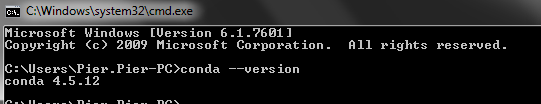
\includegraphics[scale=1]{figures/versiconda.png}
   	 \caption{Versi Anaconda Yang Digunakan}	
	\end{center}
\end{figure}
\item
Pastikan juga Kebutuhan Scikit seperti Numpy, Scipy dan Python telah terinstal. untuk mengeceknya buka CMD dan ketikan seperti gambar berikut.
\begin{figure}
	\begin{center}
   	 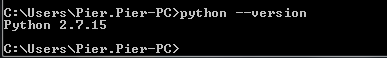
\includegraphics[scale=1]{figures/gambar.png}
   	 \caption{Versi Python Yang Digunakan}	
	\end{center}
\end{figure}
\item 
Pada CMD ketikan "conda install scikit-learn" kemudian tunggu sampai instalasi selesai.
\begin{figure}[!htbp]
	\begin{center}
   	 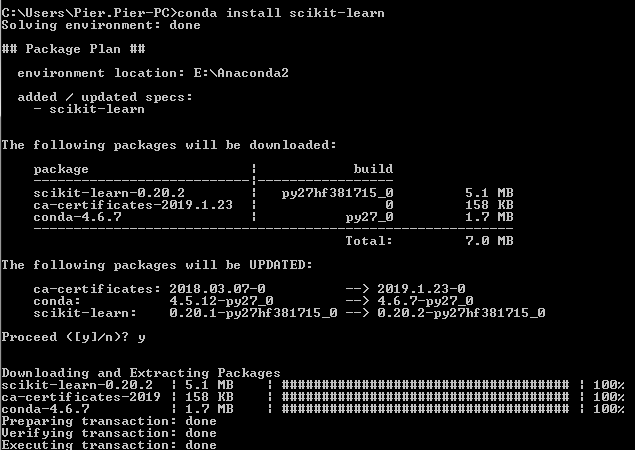
\includegraphics[scale=1]{figures/instalscikit.png}
   	 \caption{Instalasi Scikit Dari Anaconda}	
	\end{center}
\end{figure}
\item 
Setelah itu, kita akan mencoba salah satu contoh dasar penggunaan scikit pada website sebelumnya. Dan disini menggunakan contoh Multilabel classification.
\item 
Salin skrip contoh tersebut ke Text Editor Visual Code atau yang anda miliki. File ini kemudian di save dengan nama "contoh.py"
\begin{figure}
	\begin{center}
   	 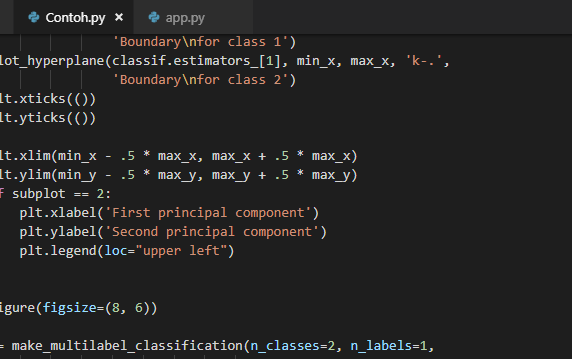
\includegraphics[scale=1]{figures/contoh.png}
   	 \caption{Contoh Skrip}	
	\end{center}
\end{figure}
\item 
Setelah tersimpan, jalankan di CMD dengan mengetikan "python contoh.py" maka akan muncul hasil seperti dibawah ini.
\begin{figure}
	\begin{center}
   	 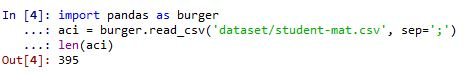
\includegraphics[scale=1]{figures/hasil1.png}
   	 \caption{Hasil Yang Muncul Di CMD}	
	\end{center}
\end{figure}
\begin{figure}
	\begin{center}
   	 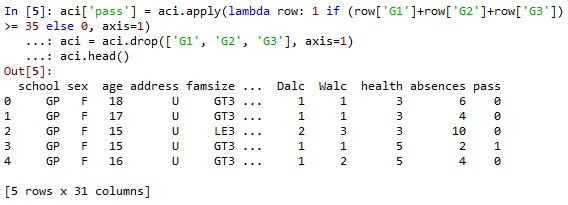
\includegraphics[scale=1]{figures/hasil2.png}
   	 \caption{Gambar Yang Muncul Dari Matplotlib}	
	\end{center}
\end{figure}
\end{enumerate}

\subsection{Mencoba Loading an example dataset, menjelaskan maksud dari tulisan tersebut dan mengartikan per baris}
\begin{enumerate}
\item
Mengimmport dataset, iris dan digit sebagai contoh data.
\begin{figure}
	\begin{center}
   	 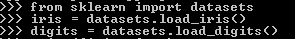
\includegraphics[scale=1]{figures/penjelasan1.png}
   	 \caption{Penjelasan }	
	\end{center}
\end{figure}
\item
Misalnya, dalam kasus dataset digit, digits.data memberikan akses ke fitur yang dapat digunakan untuk mengklasifikasikan sampel digit.
\begin{figure}
	\begin{center}
   	 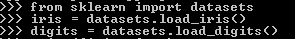
\includegraphics[scale=1]{figures/penjelasan1.png}
   	 \caption{Penjelasan 2}	
	\end{center}
\end{figure}
\item 
digit.target memberikan kebenaran dasar untuk dataset digit, yaitu angka yang sesuai dengan setiap gambar digit yang dipelajari.
\begin{figure}
	\begin{center}
   	 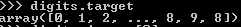
\includegraphics[scale=1]{figures/penjelasan3.png}
   	 \caption{Penjelasan 3}	
	\end{center}
\end{figure}
\item 
menggambarkan bagaimana mulai dari masalah awal seseorang dapat membentuk data untuk konsumsi di scikit-belajar.
\begin{figure}
	\begin{center}
   	 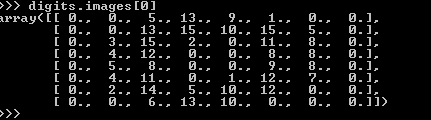
\includegraphics[scale=1]{figures/penjelasan4.png}
   	 \caption{Penjelasan 4}	
	\end{center}
\end{figure}

\end{enumerate}

<<<<<<< HEAD


\section{Teori/Annisa Fathoroni-1164067}
=======
\subsection{Mencoba Learning and predicting, menjelaskan maksud dari tulisan tersebut dan mengartikan per baris}
HARI 2

\begin{enumerate}
\item
Pada website sebelumnya, cari Learning And Predicting dan ikuti langkah -langkahnya.
\item
Buka Python Shell, atau dengan membukan Command Prompt di PC dan mengetikan python. maka akan masuk ke Python Shellnya.
\begin{figure}
	\begin{center}
   	 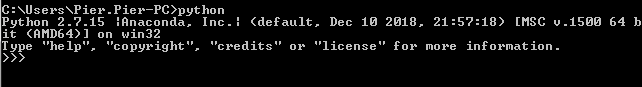
\includegraphics[scale=1]{figures/tasya1.png}
   	 \caption{Membuka Python Shell}	
	\end{center}
\end{figure}
\item
Pada python shell ketikan "from sklearn import svm" yang dimana artinya akan memanggil dan menggunakan estimator dari kelas sklearn.svm.SVC
\begin{figure}
	\begin{center}
   	 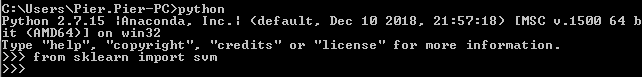
\includegraphics[scale=1]{figures/tasya2.png}
   	 \caption{Menggunakan Estimator Sklearn }	
	\end{center}
\end{figure}
\item
Kemudian, kita definisikan clf sebagai classfier, disini gamma didefinisikan secara manual
\begin{figure}
	\begin{center}
   	 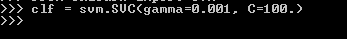
\includegraphics[scale=1]{figures/tasya3.png}
   	 \caption{Mendefinisikan Classifier }	
	\end{center}
\end{figure}
\item
Estimator clf (for classifier) pertama kali dipasang pada model. Ini dilakukan dengan melewati training set ke metode fit. Untuk training set, akan menggunakan semua gambar dari set data yang ada, kecuali untuk gambar terakhir, yang dicadangan untuk prediksi. Pada skrip dibawah memilih training set dengan sintaks Python [: -1], yang menghasilkan array baru yang berisi semua kecuali item terakhir dari digits.data
\begin{figure}
	\begin{center}
   	 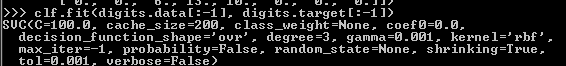
\includegraphics[scale=1]{figures/tasya4.png}
   	 \caption{Memanggil Classifier Tanpa Baris Terakhir }	
	\end{center}
\end{figure}
\item
Pada penggalan skrip dibawah, ini menunjukan prediksi nilai baru menggunakan gambar terakhir dari digits.data. Dengan prediksi akan menentukan gambar dari set pelatihan yang paling cocok dengan gambar terakhir.
\begin{figure}
	\begin{center}
   	 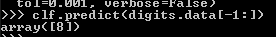
\includegraphics[scale=1]{figures/tasya5.png}
   	 \caption{Memprediksi Nilai Baru}	
	\end{center}
\end{figure}
\end{enumerate}
/AKHIR BAGIAN INSTALASI TASYA WIENDHYRA 1164086

\subsection{Mencoba Model Persistance, menjelaskan maksud dari tulisan tersebut dan mengartikan per baris} /BAGIAN TASYA WIENDHYRA 1164086
\begin{enumerate}
\item
Pada Python Shell ketikan "from sklearn import svm" artinya akan mengimport sebuah Support Vector Machine(SVM) yang merupakan algoritma classification yang akan diambil dari Scikit-Learn.
\item
Kemudian, lanjutkan dengan "from sklearn import datasets" yang artinya akan mengambil package datasets dari Scikit-Learn.
\item
ketikan, clf = svm.SVC(gamma='scale') berfungsi untuk mendeklarasikan suatu value yang bernama clf yang berisi gamma. Parameter gamma menentukan seberapa jauh pengaruh dari satu contoh training.
\item
Ketikan, X, y = iris.data, iris.target, artinya X sebagai data iris, dan y merupakan larik target.
\item
Ketikan, clf.fit(X, y) berfungsi untuk melakukan pengujian classifier. hasilnya seperti ini
\begin{figure}
	\begin{center}
   	 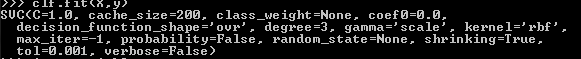
\includegraphics[scale=1]{figures/tasya7.png}
   	 \caption{Hasil Pengujian Classifier}	
	\end{center}
\end{figure}
\item
\begin{figure}
	\begin{center}
   	 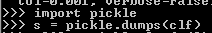
\includegraphics[scale=1]{figures/tasya8.png}
   	 \caption{Hasil Pengujian Classifier}	
	\end{center}
\end{figure}
Dari gambar diatas dapat dijelaskan bahwa akan mengimport Pickle dari Python. Pickle digunakan untuk serialisasi dan de-serialisasi struktur objek Python. Objek apa pun dengan Python dapat di-Pickle sehingga dapat disimpan di disk. kemudian menyimpan data objek ke file CLF sebelumnya dengan menggunakan function pickle.dumps(clf).
\item
Setelah mengetikan fungsi fungsi diatas, selanjutnya ketikan "clf2 = pickle.loads(s)" yang artinya pickle.loads digunakan untuk memuat data pickle dari string byte. "S" dalam loads mengacu pada fakta bahwa dalam Python 2, data dimuat dari string.
\begin{figure}
	\begin{center}
   	 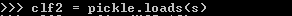
\includegraphics[scale=1]{figures/tasya9.png}
   	 \caption{Pickle Pada Python}	
	\end{center}
\end{figure}
\item
\begin{figure}
	\begin{center}
   	 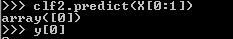
\includegraphics[scale=1]{figures/tasya10.png}
   	 \caption{Pengujian Classifier Pickle}	
	\end{center}
\end{figure}
Pada gambar diatas dilakukan pengujian nilai baru dengan menggunakan "cf2.predict(X[0:1])" dengan target asumsinya (0,1) hasilnya berbentuk array.
\item
Dalam kasus khusus scikit-learn, mungkin lebih menarik untuk menggunakan joblib (dump dan load) untuk menggantikan Pickle, yang lebih efisien pada data besar tetapi hanya bisa di Pickle ke disk dan tidak ke string. untuk menggunakan Joblib pertama ketikan "from joblib import dump , load" yang artinya akan Merekonstruksi objek Python dari file yang sudah ada.\\

dump(clf, 'filename.joblib') akan merekontruksi file CLF yang tadi sudah dideklarasikan.\\
clf = load('filename.joblib') untuk mereload model yang sudah di Pickle\\
\begin{figure}
	\begin{center}
   	 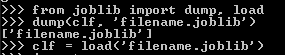
\includegraphics[scale=1]{figures/tasya11.png}
   	 \caption{Penggunaan Joblib}	
	\end{center}
\end{figure}
\end{enumerate}

\subsection{Mencoba Conventions, menjelaskan maksud dari tulisan tersebut dan mengartikan per baris}
\begin{enumerate}
\item
Import numpy as np, digunakan untuk mengimport Numpy sebagai np.\\
From sklearn import randomprojection artinya modul yang mengimplementasikan cara sederhana dan efisien secara komputasi untuk mengurangi dimensi data dengan memperdagangkan sejumlah akurasi yang terkendali (sebagai varian tambahan) untuk waktu pemrosesan yang lebih cepat dan ukuran model yang lebih kecil.
\begin{figure}
	\begin{center}
   	 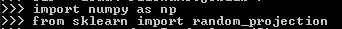
\includegraphics[scale=1]{figures/tasya12.png}
   	 \caption{Deklarasi Numpy}	
	\end{center}
\end{figure}
\item
\begin{figure}
	\begin{center}
   	 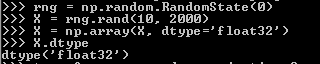
\includegraphics[scale=1]{figures/tasya13.png}
   	 \caption{Contoh Type Casting}	
	\end{center}
\end{figure}
Pada gambar diatas dapat dijelaskan bahwa :\\
rng = np.random.RandomState(0), digunakan untuk menginisialisasikan random number generator.\\
X = rng.rand(10, 2000) artinya akan merandom value antara 10 sampai 2000.\\
X = np.array(X, dtype='float32') Array numpy terdiri dari buffer memori "mentah" yang diartikan sebagai array melalui "views". Anda dapat menganggap semua array numpy sebagai tampilan. Mendeklarasikan X sebagai float32.
\item
Dalam contoh ini, X adalah float32, yang dilemparkan ke float64 oleh fittransform (X).
\begin{figure}
	\begin{center}
   	 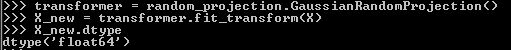
\includegraphics[scale=1]{figures/tasya14.png}
   	 \caption{Menggunakan FitTransform}
	\end{center}
\end{figure}
\item
Target regresi dilemparkan ke float64 dan target klasifikasi dipertahankan.

list(clf.predict(irisdata[:3])), akan memprediksi 3 data dari iris.\\
clf.fit irisdata, iristargetnames[iristarget] menguji classifier dengan ada targetnya yaitu irisnya sendiri.\\
list(clf.predict(irisdata[:3])), setelah diuji maka akan muncul datanya seperti dibawah ini\\
\begin{figure}
	\begin{center}
   	 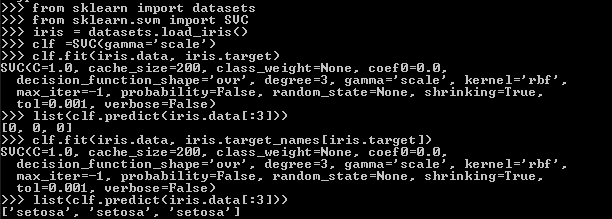
\includegraphics[scale=1]{figures/tasya15.png}
   	 \caption{Regresi Yang Dilempar}
	\end{center}
\end{figure}
Di sini, prediksi pertama () mengembalikan array integer, karena iristarget (array integer)yang digunakan sesuai. Prediksi kedua () mengembalikan array string, karena iristargetnames cocok.
\item
Refitting dan Memperbaharui Parameter

y = rngbinomial(1, 0.5, 100) , random value dengan angka binomial atau suku dua untuk y \\
clfsetparams(kernel='linear')fit(X, y) mengubahn kernel default menjadi linear \\
clfsetparams(kernel='rbf', gamma='scale')fit(X, y)  Di sini, kernel default rbf pertama kali diubah menjadi linear melalui\\ SVCsetparams () setelah estimator dibuat, dan diubah kembali ke rbf untuk mereparasi estimator dan membuat prediksi kedua.
\begin{figure}
	\begin{center}
   	 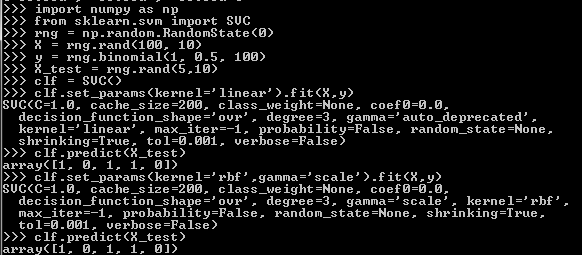
\includegraphics[scale=1]{figures/tasya16.png}
   	 \caption{Refitting dan Memperbaharui Parameter}
	\end{center}
\end{figure}
\item
MultiClass VS MultiLabel Classifier \\
from sklearn.multiclass import OneVsRestClassifier ,adalah  ketika kita ingin melakukan klasifikasi multiclass atau multilabel dan baik unutk menggunakan OneVsRestClassifier per kelas. Untuk setiap classifier, kelas tersebut dipasang terhadap semua kelas lainnya. (Ini cukup jelas dan itu berarti bahwa masalah klasifikasi multiclass / multilabel dipecah menjadi beberapa masalah klasifikasi biner).\\
from sklearn.preprocessing import LabelBinarizer ,adalah kelas utilitas untuk membantu membuat matriks indikator label dari daftar label multi-kelas\\
Dalam gambar dibawah, classifier cocok pada array 1d label multiclass dan oleh karena itu metode predict () memberikan prediksi multiclass yang sesuai.
\begin{figure}
	\begin{center}
   	 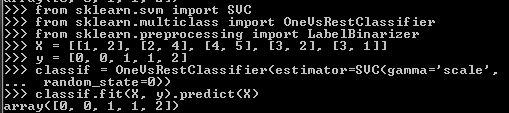
\includegraphics[scale=1]{figures/tasya17.png}
   	 \caption{MultiClass Classifier}
	\end{center}
\end{figure}
\item
Di sini, classifier cocok () pada representasi label biner 2d dari y, menggunakan LabelBinarizer. Dalam hal ini predict () mengembalikan array 2d yang mewakili prediksi multilabel yang sesuai.
\begin{figure}
	\begin{center}
   	 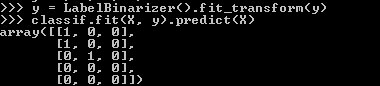
\includegraphics[scale=1]{figures/tasya18.png}
   	 \caption{MultiClass Classifier biner 2D}
	\end{center}
\end{figure}
\item
from sklearn.preprocessing import MultiLabelBinarizer , artinya Transformasi antara iterable dari iterables dan format multilabel.\\
Dalam hal ini, penggolongnya sesuai pada setiap instance yang diberi beberapa label. MultiLabelBinarizer digunakan untuk membuat binarize array 2d dari multilabel agar sesuai. Hasilnya, predict () mengembalikan array 2d dengan beberapa label yang diprediksi untuk setiap instance.
\begin{figure}
	\begin{center}
   	 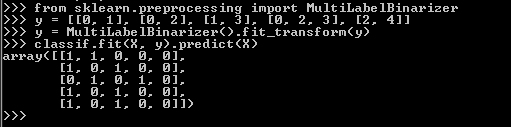
\includegraphics[scale=1]{figures/tasya19.png}
   	 \caption{MultiLabel Classifier}
	\end{center}
\end{figure}
\end{enumerate}
/AKHIR BAGIAN PEGUJIAN TASYA WIENDHYRA 1164086

\section{Penanganan Error} /BAGIAN TASYA WIENDHYRA 1164086
HARI KEDUA
\begin{enumerate}
	\item
	Berikut ini merupakan eror yang ditemui pada saat melakukan percobaan skrip.
\begin{figure}
	\begin{center}
   	 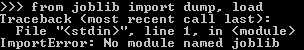
\includegraphics[scale=1]{figures/eror2.png}
   	 \caption{Eror Import}
	\end{center}
\end{figure}
	\item
Pada gambar eror diatas, kode erornya adalah "ImportError: No Module Named" artinya mengalami masalah saat mengimpor modul yang ditentukan.
	\item
Solusinya bisa dilakukan seperti berikut :\\
eror diats terjadi dikarenakan Library Joblib belum terinstal pada PC. Maka dari itu sekarang kita harus menginstalnya dulu.
	\item
Buka CMD, kemudian ketikan "pip install joblib" tunggu sampai instalasi berhasil seperti gambar berikut.
\begin{figure}
	\begin{center}
   	 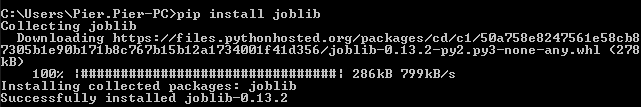
\includegraphics[scale=1]{figures/solusi2.png}
   	 \caption{Instal Library Joblib}
	\end{center}
\end{figure}
	\item
Apabila sudah terinstall, dapat dilakukan lagi import library joblib, maka akan berhasil seperti dibawah berikut
\begin{figure}
	\begin{center}
   	 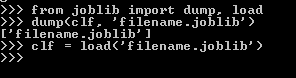
\includegraphics[scale=1]{figures/solusi2_1.png}
   	 \caption{Berhasil Import Library Joblib}
	\end{center}
\end{figure}
\end{enumerate}
/AKHIR BAGIAN PENANGANAN EROR TASYA WIENDHYRA 1164086

\section{Teori}
>>>>>>> f7e668a111f4077890da4ffc952276254d03059b
Teori mencakup resume dari beberapa pembahasan. yaitu :
\begin{enumerate}
\item Kecerdasan Buatan
\begin{itemize}
\item Definisi Kecerdasan Buatan.
\par Jadi yang dimaksud dengan  kecerdasan buatan yaitu  salah satu dari cabang Ilmu pengetahuan yang kita punya dan  berhubungan juga dengan pemanfaatan mesin yaitu untuk dapat memecahkan suatu  persoalan yang rumit dengan  menggunakan cara yang lebih manusiawi.
\par Jadi yang dimaksud dengan supervised learning  adalah pembelajaran mesin yang diawasi menciptakan model yang melancarkan prediksi berdasarkan bukti adanya ketidakpastian. Algoritma pembelajaran yang diawasi memerlukan seperangkat data masukan dan tanggapan yang diketahui terhadap data (output) dan melatih model untuk menghasilkan prediksi yang masuk akal untuk respon terhadap data baru. Sedangkan untuk klasifikasi yaitu nilai output yang  bernilai diskrit (kelas) dan Bertujuan mengklasifikasi data baru dengan akurat diawasi dengan menggunakan teknik klasifikasi dan regresi untuk mengembangkan model prediktif. Yang dimaksud dengan regresi adlah nilai output yang bernilai kontinu (riil), Bertujuan memprediksi output dengan akurat untuk data baru.
\par Unsupervised learning tidak menggunakan data latih atau data training untuk melakukan prediksi maupun klasifikasi. Berdasarkan model matematisnya, algoritma ini tidak memiliki target variabel. Salah satu tujuan dari algoritma ini adalah mengelompokkan objek yang hampir sama dalam suatu area tertentu. Dan yang dimaksud dengan  Dataset adalah objek yang merepresentasikan data dan relasinya di memory. Strukturnya mirip dengan data di database. Dataset berisi koleksi dari datatable dan datarelation. Sedangkan testing set digunakan untuk mengukur sejauh mana classifier berhasil melakukan klasifikasi dengan benar. Dan training set digunakan oleh algoritma klassifikasi untuk membentuk sebuah model classifier. Model yang dimaksud ini merupakan representasi pengetahuan yang akan digunakan untuk prediksi kelas data baru yang belum pernah ada.
\end{enumerate} 

<<<<<<< HEAD
Kecerdasan buatan (Artificial Intelligence) atau disingkat menjadi AI adalah suatu pengetahuan yang membuat suatu komputer dapat menirkan  kecerdasan manusia sehingga diharapkan atau diinginkan komputer dapat melakukan hal-hal yang apabila dikerjakan manusia memerlukan kecerdasan. Misalnya melakukan penalaran untuk mencapai suatu kesimpulan atau melalukan translasi dari satu bahasa manusia ke bahasa manuasi yang lain.


\item Perkembangan Kecerdasan Buatan
\begin{figure}[ht]
\centering
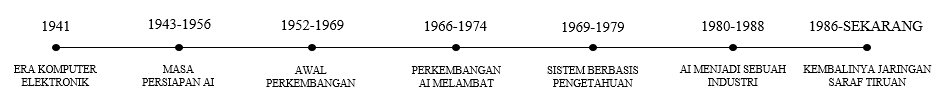
\includegraphics[scale=0.5]{figures/Screenshot_1.png}
\caption{capturing}
\label{perkembangan}
\end{figure}

Ditemukannya pertama kali alat penyimpanan dan pemrosesan informasi yang disebut komputer elektronik. Tahun 1943, Warren McCulloch dan Walter Pitts berhasil membuat suatu model saraf tiruan di mana setiap neuron digambarkan sebagai ‘on’ dan ‘off’. Pada tahun 1950, Norbert Wiener membuat penelitian mengenai prinsip-prinsip teori feedback. Pada tahun 1956, John McCarthy meyakinkan Minsky, Claude Shannon, dan Nathaniel Rochester untuk membantunya melakukan penelitian dalam bidang automata, jaringan saraf, dan pembelajaran intelijensia. Mereka mengerjakan proyek ini selama 2 bulan di Universitas Dartmouth. Hasilnya adalah program yang mampu berpikir non-numerik dan menyelesaikan masalah pemikiran, yang dinamakan Principia Mathematica. Hal ini menjadikan McCarthy disebut sebagai father of Artificial Intelligence/ Bapak Kecerdasan Buatan.

Pada tahun 1958, McCarthy di MIT AI Lab mendefinisikan bahasa pemrograman tingkat tinggi yaitu LISP, yang sekarang mendominasi pembuatan program-program AI. Kemudian, McCarthy membuat program yang dinamakan programs with common sense. Pada tahun 1959, Program komputer General Problem Solver berhasil dibuat oleh Herbert A. Simon, J.C. Shaw, dan Allen Newell. Program ini dirancang untuk memulai penyelesaian masalah secara manusiawi. Pada tahun yg sama Nathaniel Rochester dari IBM dan para mahasiswanya merilis program AI yaitu geometry theorem prover. Pada tahun 1963, program yang dibuat James Slagle mampu menyelesaikan masalah integral tertutup untuk mata kuliah Kalkulus. Pada tahun 1968, program analogi buatan Tom Evan menyelesaikan masalah analogi geometri yang ada pada tes IQ.

Perkembangan AI melambat disebabkan adanya beberapa kesulitan yang di hadapi seperti  Program-program AI yang bermunculan hanya mengandung sedikit atau bahkan tidak mengandung sama sekali pengetahuan pada subjeknya, banyak terjadi kegagalan pada pembuatan program AI, terdapat beberapa batasan pada struktur dasar yang digunakan untuk menghasilkan perilaku intelijensia. Pada tahun 1960an, Ed Feigenbaum, Bruce Buchanan, dan Joshua Lederberg merintis proyek DENDRAL yaitu program untuk memecahkan masalah struktur molekul dari informasi yang didapatkan dari spectometer massa. Pada tahun 1986, program ini telah berhasil menghemat 40 juta dolar per tahun. Pada tahun 1988, kelompok AI di DEC menjalankan 40 sistem pakar. Hampir semua perusahaan besar di USA mempunyai divisi Ai sendiri yang menggunakan ataupun mempelajari sistem pakar. Perusahaan yang sejak tahun 1982 hanya menghasilkan beberapa juta US dollar per tahun meningkat menjadi 2 milyar US dollar per tahun pada tahun 1988.

Meskipun bidang ilmu komputer menolak jaringan saraf tiruan setelah diterbitkannya buku ‘Perceptrons’ karangan Minsky dan Papert, tetapi para ilmuwan masih mempelajari bidang ilmu tersebut dari sudut pandang yang lain, yaitu fisika. Ahli fisika seperti Hopfield (1982) menggunakan teknik-teknik mekanika statistika untuk menganalisa sifat-sifat penyimpanan dan optimasi pada jaringan saraf. Para ahli psikolog, David Rumhelhart dan Geoff Hinton melanjutkan penelitian mengenai model jaringan saraf pada memori. Pada tahun 1985-an sedikitnya empat kelompok riset menemukan algoritma Back-Propagation. Algoritma ini berhasil diimplementasikan ke dalam ilmu bidang komputer dan psikologi.

\end{itemize}
\item Supervised Learning, Klasifikasi dan Regresi.
\begin{itemize}
\item Supervised learning adalah sebuah pendekatan dimana sudah terdapat data yang dilatih, dan terdapat variable yang ditargetkan sehingga tujuan dari pendekatan ini adalah mengkelompokan suatu data ke data yang sudah ada.

\item Dalam klasifikasi, keluaran dari setiap data adalah bilangan bulat atau diskrit. Misalnya pengambilan keputusan untuk main sepak bola atau tidak maka keluaran bisa diubah kedalam bilangan bulat 1 (main bola), dan -1 (tidak main). Regresi, keluaran dari setiap data dalah bilangan kontinu. Misalnya peramalan harga rumah berdasarkan lokasi, umur rumah dan luas rumah, maka keluarannya berupa bilangan kontinu berupa bilangan Rp 120 juta, Rp 100 juta atau Rp 51 juta.

\begin{figure}[ht]
\centering
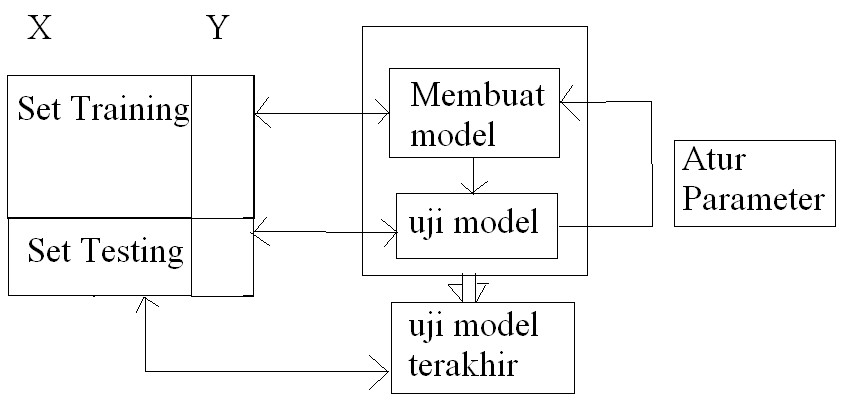
\includegraphics[scale=0.5]{figures/Screenshot_2.jpg}
\caption{install anaconda 2}
\label{contoh}
\end{figure}

\end{itemize}
\end{enumerate} 


\section{Instalasi/Annisa Fathoroni-1164067)}
Untuk Instalasinya mencakup beberapa pembahasan dan tutorial. yaitu :
\begin{enumerate}
\item Instalasi Scikit-Learn Dari Anaconda 
\begin{itemize}
\item Instalasi Anaconda
\begin{enumerate}

\begin{figure}[ht]
\centering
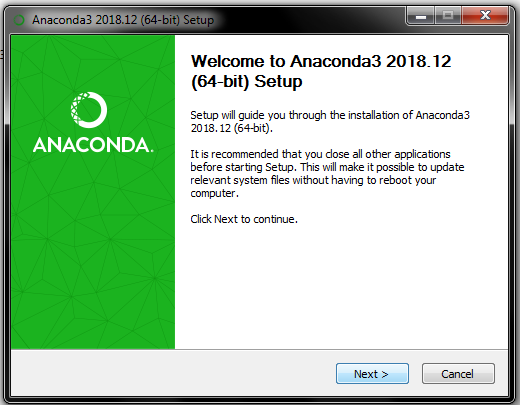
\includegraphics[scale=0.5]{figures/1.png}
\caption{capturing}
\label{proses instalasi}
\end{figure}

\begin{figure}[ht]
\centering
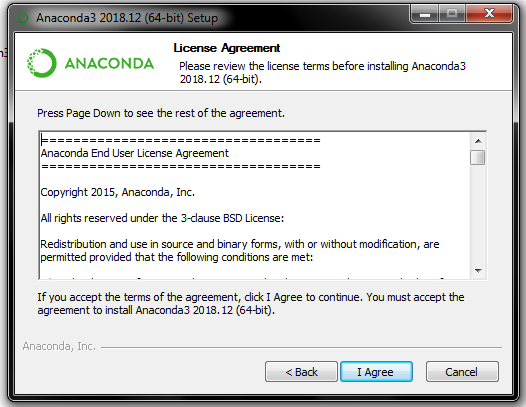
\includegraphics[scale=0.5]{figures/2.png}
\caption{capturing}
\label{proses instalasi}
\end{figure}

\begin{figure}[ht]
\centering
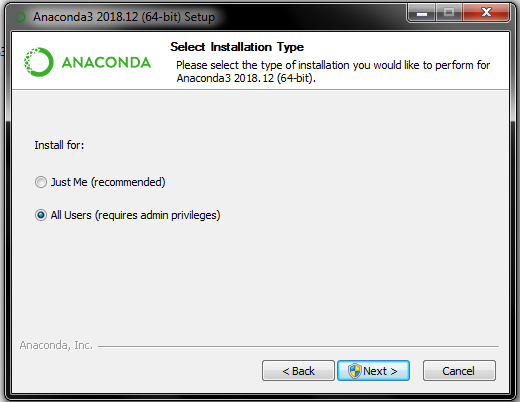
\includegraphics[scale=0.5]{figures/3.png}
\caption{capturing}
\label{proses instalasi}
\end{figure}

\begin{figure}[ht]
\centering
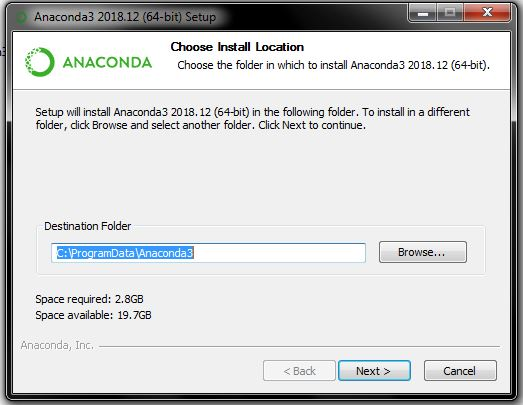
\includegraphics[scale=0.5]{figures/4.jpg}
\caption{capturing}
\label{proses instalasi}
\end{figure}

\begin{figure}[ht]
\centering
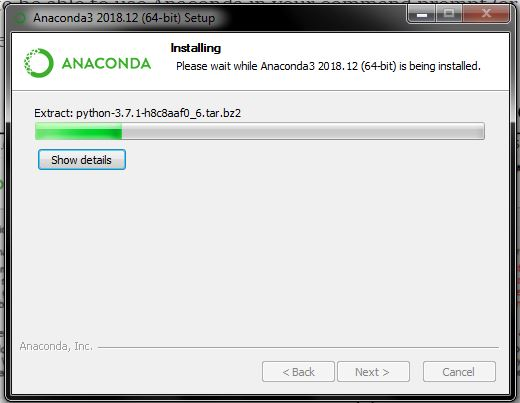
\includegraphics[scale=0.5]{figures/6.jpg}
\caption{capturing}
\label{proses instalasi}
\end{figure}

\begin{figure}[ht]
\centering
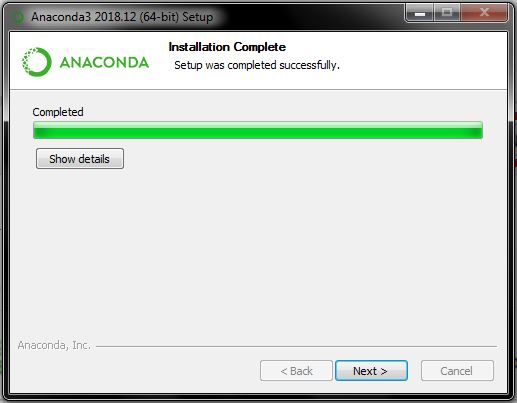
\includegraphics[scale=0.5]{figures/7.jpg}
\caption{capturing}
\label{proses instalasi}
\end{figure}

\begin{figure}[ht]
\centering
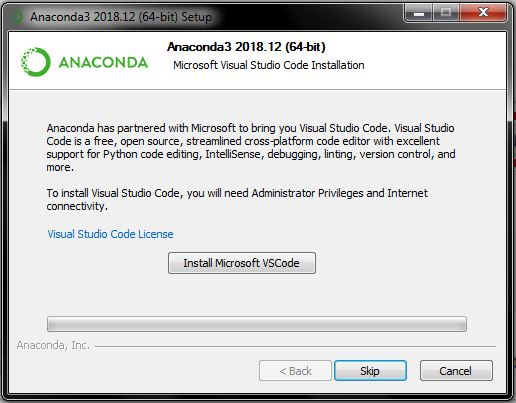
\includegraphics[scale=0.5]{figures/8.jpg}
\caption{capturing}
\label{proses instalasi}
=======
\section
\item 
Mencoba Learning and predicting, menjelaskan maksud dari tulisan tersebut dan mengartikan per baris[hari ke 2](10)
\begin{figure}
	\begin{center}
   	 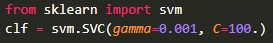
\includegraphics[scale=0.5]{figures/cahya1.png}
   	 \caption{capturing}	
	\end{center}
>>>>>>> f7e668a111f4077890da4ffc952276254d03059b
\end{figure}
Pada gambar diatas dapat dijelaskan bahwa :\\
Baris yang pertama  kita memasukkan dan memanggil svm dari sklearn.\\
Baris yang kedua  kita membuat variable.\\
\item)
\begin{figure}
	\begin{center}
   	 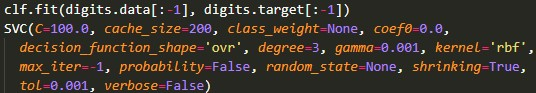
\includegraphics[scale=0.5]{figures/cahya2.png}
   	 \caption{capturing}	
	\end{center}
\end{figure}
Pada gambar diatas dapat dijelaskan bahwa :\\
Baris yang pertama itu clf dipasang pada model fit metode.\\
Baris yang kedua kita implementasikan klasifikasi dukungan vektor.\\
\item 
\begin{figure}
	\begin{center}
   	 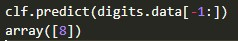
\includegraphics[scale=0.5]{figures/cahya3.png}
   	 \caption{capturing}	
	\end{center}
\end{figure}
Pada gambar diatas dapat dijelaskan bahwa :\\
Baris yang pertama itu untuk prediksi nilai baru.\\
Baris yang kedua untuk set array.\\

<<<<<<< HEAD
\begin{figure}[ht]
\centering
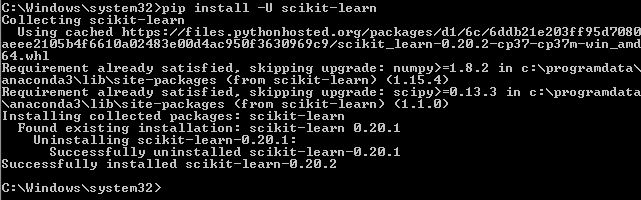
\includegraphics[scale=0.5]{figures/12.jpg}
\caption{capturing}
\label{proses instalasi}
\end{figure}

\item Setelah proses download selesai, run package yang telah didownload lalu next.
\item Pilih 'I Agree' untuk menyetujui persyaratan dan peraturan mengenai aplikasi ini.
\item Lalu, pilih 'All Users' untuk dapat diakses oleh semua user, dan pilih "Just Me' hanya untuk dapat diakses oleh 1 user pc.
\item Kemudian, pilih penyimpanan package.
\item Ceklis pada bagian cek box pertama untuk otomatis pengaturan dan penambahan enviroment variabel pada PATH dan cek box kedua untuk register anaconda sistem.
\item Proses instalasi
\item Lalu pada proses ini, skip untuk mempercepat proses penginstalan.
\item Proses instalasi selesai.
\item Setelah proses instalasi selesai, cek penginstalan conda dan python.
\item Lalu install scikit dengan perintah 'pip install -U scikit-learn" atau 'conda install scikit-learn'
\end{enumerate}
\end{itemize}

\item Loading an Example Dataset
\begin{figure}[ht]
\centering
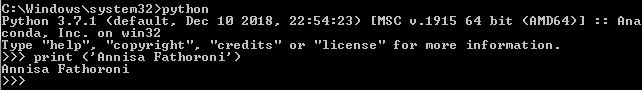
\includegraphics[scale=0.5]{figures/Capture2.jpg}
\caption{capturing}
\label{uji coba}
=======
\end{enumerate}

\section
\item 
mencoba Model persistence, menjelaskan maksud dari tulisan tersebut dan mengartikan per baris[hari ke 2](10)
\begin{figure}
	\begin{center}
   	 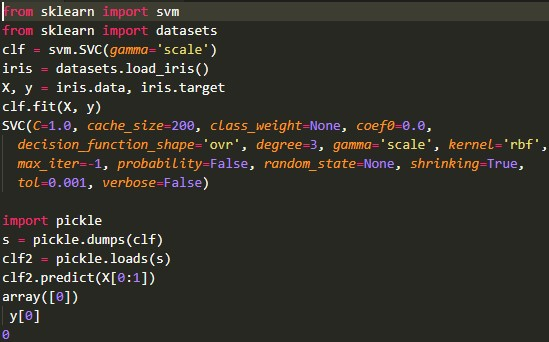
\includegraphics[scale=0.5]{figures/cahya4.png}
   	 \caption{capturing}	
	\end{center}
>>>>>>> f7e668a111f4077890da4ffc952276254d03059b
\end{figure}
Pada gambar diatas dapat dijelaskan bahwa :\\
Baris yang pertama kita memasukkan dan memanggil datasets dari sklearn.\\
Baris yang kedua kita memasukkan dan memanggil svm dari sklearn.\\
Baris yang ketiga kita  membuat variable clf.\\
Baris yang keempat kita  membuat variable iris.\\
Baris yang kelima kita  membuat variable x, y.\\
Baris yang keenam  clf dipasang pada model fit metode.\\
Baris yang ke tujuh kita  implementasikan klasifikasi dukungan vektor.\\
Baris yang kedelapan kita memanggil library pickle.\\
Baris yang kesembilan untuk  membuat variable s.\\
Baris yang kesepuluh untuk  membuat variable clf2.\\
Baris yang keseblas untuk  prediksi nilai baru.\\
Baris yang keduabelas untuk  set array.\\

\end{enumerate}


\item 
Mencoba Conventions, menjelaskan maksud dari tulisan tersebut dan mengartikan per baris[hari ke 2](10)
\begin{figure}
	\begin{center}
   	 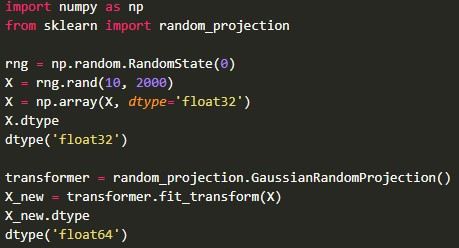
\includegraphics[scale=0.5]{figures/cahya5.png}
   	 \caption{capturing}	
	\end{center}
\end{figure}
<<<<<<< HEAD

\item Baris 1:
Memanggil data dari sklearn.
\item Baris 2:
Terdapat variabel 'iris', dimana variabel iris memanggil datasets dan di dalamnya akan memproses digits.
\item Baris 3:
Kemudian ada variabel lainnya 'digits' yang digunakan untuk memanggil dataset dan di dalamnya akan memproses digits.
\item Kemudian untuk perintah Print( digits.data ) untuk menampilkan output dari hasil variabel digits dan akan berupa data.

\end{enumerate}

\begin{itemize}
\item Mencoba Learning and Predicting.

\begin{figure}[ht]
\centering
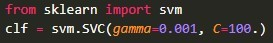
\includegraphics[scale=0.5]{figures/Capture3.jpg}
\caption{capturing}
\label{loading an example dataset}
\end{figure}

Baris 1 = Memasukkan dan memanggil SVM dari sklearn.

Baris 2 = Membuat variabel.

\begin{figure}[ht]
\centering
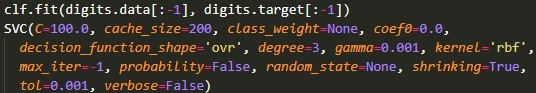
\includegraphics[scale=0.5]{figures/Capture4.jpg}
\caption{capturing}
\label{loading an example dataset}
\end{figure}

Baris 1 = clf dipasang pada model fit metode.

Baris 2 = Mengimplementasikan klasifikasi dukungan vektor.

\begin{figure}[ht]
\centering
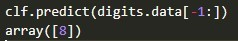
\includegraphics[scale=0.5]{figures/Capture5.jpg}
\caption{capturing}
\label{loading an example dataset}
\end{figure}

Baris 1 = Prediksi nilai baru.

Baris 2 = set array.

\end{itemize}

\begin{itemize}
\item Model Persistence

\begin{figure}[ht]
\centering
\includegraphics[scale=0.5]{figures/Capture6.jpg}
\caption{capturing}
\label{loading an example dataset}
\end{figure}

Baris 1 = Memasukkan dan memanggil datasets dari sklearn.

Baris 2 = Memasukkan dan memanggil SVM dari sklearn.

Baris 3 = Membuat variable clf.

Baris 4 = Membuat variable iris.

Baris 5 = Membuat variable x dan y.

Baris 6 = clf dipasang pada model fit metode.

Baris 7 = Mengimplementasikan klasifikasi dukungan vektor.

Baris 8 = Memanggil library pickle.

Baris 9 = Membuat variable s.

Baris 10 = Membuat variable clf2.

Baris 11 = Memprediksikan nilai baru.

Baris 12 = Set array.

\end{itemize}

\begin{itemize}
\item Conventions

\begin{figure}[ht]
\centering
\includegraphics[scale=0.5]{figures/Capture7.jpg}
\caption{capturing}
\label{loading an example dataset}
\end{figure}

Baris 1 = Memasukkan dan memanggil numpy sebagai np.

Baris 2 = Memasukkan dan memanggil randomprojection dari sklearn.

Baris 3 = Membuat variable rng.

Baris 4 = Membuat variable rng.

Baris 5 = Membuat variable x.

Baris 6 = Proses pemanggilan variable x.

Baris 7 = Proses pemanggilan dtype.

Baris 8 = Membuat variable tranformer.

Baris 9 = Membuat variable xnew.

Baris 10 = Proses pemanggilan xnew.

Baris 11 = Pemanggilan dtype.

\end{itemize}

\section{Penanganan Error/Annisa Fathoroni-1164067)}
Untuk penanganan error mencakup beberapa pembahasan dan tutorial. yaitu :
\begin{enumerate}
\item Screenshoot Error

\begin{figure}[ht]
\centering
\includegraphics[scale=0.5]{figures/Capture8.png}
\caption{capturing}
\label{loading an example dataset}
\end{figure}

\item Kode Error dan Jenis Errornya

SyntaxError: invalid syntax

\item Solusi Pemecahan Error.

\begin{figure}[ht]
\centering
\includegraphics[scale=0.5]{figures/Capture9.png}
\caption{capturing}
\label{loading an example dataset}
\end{figure}
=======
Pada gambar diatas dapat dijelaskan bahwa :\\
Baris yang pertama kita memasukkan dan memanggil numpy sebagai np.\\
Baris yang kedua kita memasukkan dan memanggil random_projection dari sklearn.\\
Baris yang ketiga kita  membuat variable rng.\\
Baris yang keempat untuk  membuat variable rng.\\
Baris yang kelima untuk  membuat variable x.\\
Baris yang keenam untuk  pemanggilan variable x.\\
Baris yang ketujuh untuk pemanggilan dtype.\\
Baris yang kedelapan kita membuat variable tranformer.\\
Baris yang kesembilan kita membuat variable x_new.\\
Baris yang kesempulah untuk  pemanggilan x_new.\\
Baris yang keseblas untuk  pemanggilan dtype.\\
>>>>>>> f7e668a111f4077890da4ffc952276254d03059b

\end{enumerate}